\section{Circuitos aritméticos}


\frame{
	\frametitle{Circuitos aritméticos}

	\begin{block}{}
		\begin{itemize}
			\item Circuitos que realizam operações
			aritméticas com números binários.
			\item São utilizados, principalmente, para construir a \textbf{ULA} - Unidade Lógico Aritmética.
			\item Geralmente realizam operações de soma e subtração.
		\end{itemize}
	\end{block}
}

\frame{
	\frametitle{Circuitos somadores - Meio somador}

	\begin{block}{Meio Somador}
		\begin{itemize}
			\item Possibilita a soma de 2 números binários de 1 bit.
			\item Entradas: 2 bits.
			\item Saídas: Soma + \textit{Carry}.
		\end{itemize}
	\end{block}
	
	\bigskip
	
%	\renewcommand{\arraystretch}{1}
	\centering
	\begin{adjustbox}{totalheight=0.6\textheight-2\baselineskip}
	\begin{tabular}{cc|cc}
		\toprule
		$ A $ & $ B $ & $ S $ & $ C $ \\ \midrule %\cmidrule(r{0.8em}){1-2}\cmidrule(l{-0.4em}){3-4}
		0 & 0 & 0 & 0 \\
		0 & 1 & 1 & 0 \\
		1 & 0 & 1 & 0 \\
		1 & 1 & 0 & 1 \\ \bottomrule
	\end{tabular}
	\end{adjustbox}
}

\frame{
	\frametitle{Circuitos somadores - Meio somador}
	
	\setmyunit{2cm}
	
	\centering
	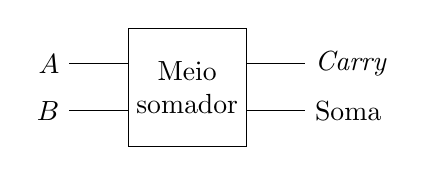
\begin{tikzpicture}[scale=1.5]
		\draw (0,0) rectangle node[text width=1.5cm, align=center] {Meio somador} ++(1,1);
		\draw (-0.5,0.3) node[left] {$ B $} -- ++(0.5,0) (-0.5,0.7) node[left] {$ A $} -- ++(0.5,0) (1,0.3) -- ++(0.5,0) node[right] {Soma} (1,0.7) -- ++(0.5,0) node[right] {\textit{Carry}};
	\end{tikzpicture}
	
}

\frame{
\frametitle{Circuitos somadores - Meio somador}

\begin{center}

\begin{karnaugh-map}[2][2][1][$A$][$B$]
\manualterms{0,1,1,0}
\implicant{1}{1}
\implicant{2}{2}
\end{karnaugh-map}
\end{center}

\vspace{-0.5cm}

\begin{block}{Expressão simplificada}
	\[ S = {\color{orange} A \oplus B } \]
\end{block}
}

\frame{
\frametitle{Circuitos somadores - Meio somador}

\begin{center}

\begin{karnaugh-map}[2][2][1][$A$][$B$]
\manualterms{0,0,0,1}
\implicant{3}{3}
\end{karnaugh-map}
\end{center}

\vspace{-0.5cm}

\begin{block}{Expressão simplificada}
	\[ C = {\color{red} A\cdot B} \]
\end{block}
}

\frame{
	\frametitle{Circuitos somadores - Meio somador}
	
	\setmyunit{2cm}
	
	\centering
	\begin{circuitikz}
		\node[xor port] (xor1) at (0,0) {};
		\node[and port] (and1) at (0,-1) {};
		
		\draw (xor1.in 1) to[short,-*] ++(-0.1,0) -- ++(-0.4,0) node[left] {$ A $} (xor1.in 2) to[short,-*] ++(-0.3,0) -- ++(-0.2,0) node[left] {$ B $} (xor1.in 1) ++(-0.1,0) |- (and1.in 1) (xor1.in 2) ++(-0.3,0) |- (and1.in 2) (xor1.out) -- ++(0.5,0) node[right] {$ S $} (and1.out) -- ++(0.5,0) node[right] {$ C $};
	\end{circuitikz}
%	\centerline{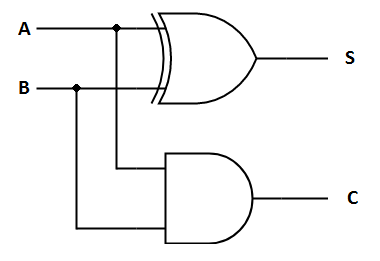
\includegraphics[width=0.5\linewidth]{Figuras/Ch9/meiosomador.png}}
}

\frame{
	\frametitle{Circuitos somadores - Somador completo}
	\begin{block}{Somador Completo}
		\begin{itemize}
			\item Possibilita a soma de 2 números binários de 1 bit + o carry anterior.
			\item Entradas: 2 bits + \textit{Carry in}.
			\item Saídas: Soma + \textit{Carry out}.
		\end{itemize}
	\end{block}

	\bigskip

	\centering
	\begin{tabular}{ccc|cc}
		\toprule
		$ A $ & $ B $ & $ C_{in} $ & $ S $ & $ C_{out} $ \\ \midrule %\cmidrule(r{1.4em}){1-3}\cmidrule(l{-0.2em}){4-5}
		0 & 0 & 0 & 0 & 0 \\
		0 & 0 & 1 & 1 & 0 \\
		0 & 1 & 0 & 1 & 0 \\
		0 & 1 & 1 & 0 & 1 \\
		1 & 0 & 0 & 1 & 0 \\
		1 & 0 & 1 & 0 & 1 \\
		1 & 1 & 0 & 0 & 1 \\
		1 & 1 & 1 & 1 & 1 \\ \bottomrule
	\end{tabular}
}

\frame{
	\frametitle{Circuitos somadores - Somador completo}
	
	\setmyunit{2cm}
	
	\centering
	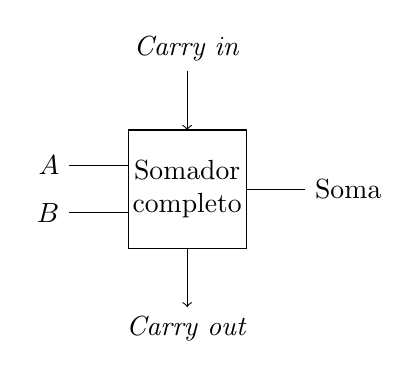
\begin{tikzpicture}[scale=1.5]
	\draw (0,0) rectangle node[text width=1.5cm, align=center] {Somador completo} ++(1,1);
	\draw (-0.5,0.3) node[left] {$ B $} -- ++(0.5,0) (-0.5,0.7) node[left] {$ A $} -- ++(0.5,0) (1,0.5) -- ++(0.5,0) node[right] {Soma};
	\draw[->] (0.5,1.5) node[above] {\textit{Carry in}} -- ++(0,-0.5);
	\draw[->] (0.5,0) -- ++(0,-0.5) node[below] {\textit{Carry out}};
	\end{tikzpicture}
	
%	\centerline{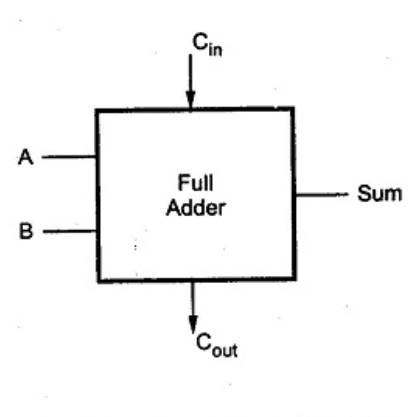
\includegraphics[width=0.5\linewidth]{Figuras/Ch9/somadorcompletobloco.PNG}}
}

\frame{
\frametitle{Circuitos somadores - Somador completo}

\begin{center}

\begin{karnaugh-map}[4][2][1][$AB$][$C_{in}$]
\manualterms{0,1,1,0,1,0,0,1}
\implicant{1}{1}
\implicant{2}{2}
\implicant{4}{4}
\implicant{7}{7}
\end{karnaugh-map}
\end{center}

\vspace{-0.5cm}

\begin{block}{Expressão simplificada}
	\[ S = {\color{orange} A \oplus B \oplus C_{in}} \]
\end{block}
}

\frame{
\frametitle{Circuitos somadores - Somador completo}

\begin{center}

\begin{karnaugh-map}[4][2][1][$AB$][$C_{in}$]
\manualterms{0,0,0,1,0,1,1,1}
\implicant{3}{7}
\implicant{5}{7}
\implicant{7}{6}
\end{karnaugh-map}
\end{center}

\vspace{-0.5cm}

\begin{block}{Expressão simplificada}
	\[ C_{out} = {\color{red} A\cdot B} + {\color{green} B\cdot C_{in}} + {\color{YellowOrange} A\cdot C_{in}} \]
\end{block}
}

\frame{
	\frametitle{Circuitos somadores - Somador completo}
	\setmyunit{2cm}
	
	\centering
	\begin{circuitikz}
		\node[xor port] (xor1) at (0.5,0) {};
		\node[and port] (and1) at (0.5,-1) {};
		\node[and port] (and2) at (0.5,-1.75) {};
		\node[and port] (and3) at (0.5,-2.5) {};
		
		\node[xor port] (xor2) at (1.5,-0.25) {};
		\node[or port,number inputs=3] (or1) at (1.5,-1.75) {};
		
		\coordinate (a) at (-1.5,0.5);
		\coordinate (b) at (-1.1,0.5);
		\coordinate (c) at (-0.7,0.5);
		
		\draw (a) node[above] {$ A $} |- (and2.in 1) (a|-xor1.in 1) to[short,*-*] (a|-and1.in 1) (xor1.in 1) -- (a|-xor1.in 1) (and1.in 1) -- (a|-and1.in 1)
		(b) node[above] {$ B $} |- (and3.in 1) (b|-xor1.in 2) to[short, *-*] (b|-and1.in 2) (xor1.in 2) -- (b|-xor1.in 2) (and1.in 2) -- (b|-and1.in 2)
		(c) node[above] {$ C_{in} $} |- (and3.in 2) (c|-xor2.in 2) to[short,*-*] (c|-and2.in 2) (xor2.in 2) -- (c|-xor2.in 2) (and2.in 2) -- (c|-and2.in 2)
		(xor1.out) |- (xor2.in 1)
		(and1.out) -| (or1.in 1)
		(and2.out) -- (or1.in 2)
		(and3.out) -| (or1.in 3)
		(xor2.out) -- ++(0.5,0) node[right] {$ S $}
		(or1.out) -- ++(0.5,0) node[right] {$ C_{out} $};
	\end{circuitikz}
%	\centerline{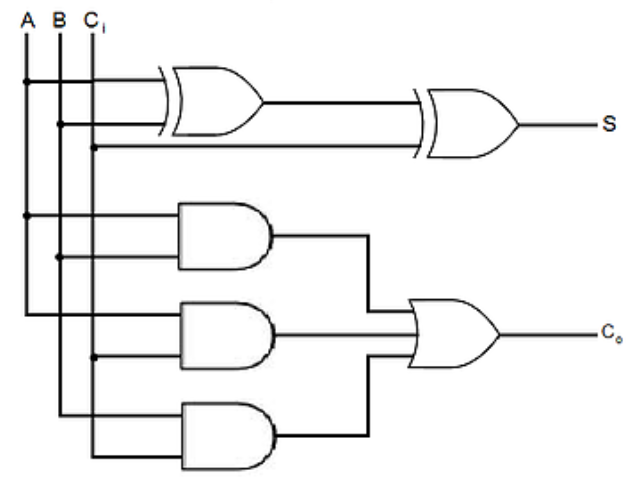
\includegraphics[width=0.7\linewidth]{Figuras/Ch9/somadorcompleto.PNG}}
}

\frame{
	\frametitle{Circuitos somadores - Somador de $ n $ bits}
	\begin{block}{\textbf{Ex.:} Somador de 4 bits}
		\begin{itemize}
			\item Utiliza-se 4 somadores completos, um para cada bit.
			\item Para o LSB pode ser utilizado um meio somador - \textbf{Por quê?}
			\item Conecta-se cada $C_{out}$ no $C_{in}$ do próximo bit.
		\end{itemize}
	\end{block}

	\centerline{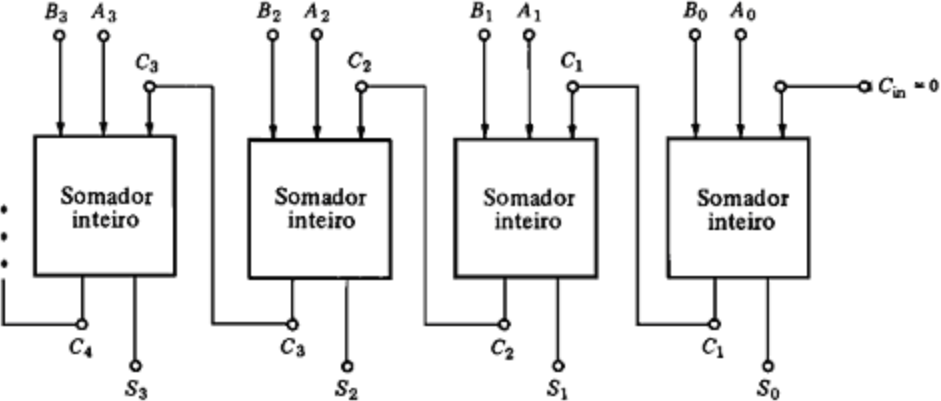
\includegraphics[width=0.9\linewidth]{Figuras/Ch9/somadornbits.PNG}}
}

\frame{
	\frametitle{Circuitos somadores - Somador completo a partir de meio somadores}
	\begin{block}{}
		\begin{itemize}
			\item Meio somador:
			\begin{align*}
				S &= {\color{orange} A \oplus B}\\
				C &= {\color{red} A\cdot B}
			\end{align*}
			\item Somador completo:
			\begin{align*}
				S 		&= {\color{orange} A \oplus B \oplus C_{in}}\\[0.5em]
				C_{out} &= \notted{A}\cdot B\cdot C_{in} + A\cdot \notted{B}\cdot C_{in} + A\cdot B\cdot \notted{C_{in}} + A\cdot B\cdot C_{in} \\
						&= {\color{red} C_{in}(A \oplus B) + A\cdot B}
			\end{align*}
		\end{itemize}
	\end{block}

}

\frame{
	\frametitle{Circuitos Somadores - Somador completo a partir de meio somadores}
	\centerline{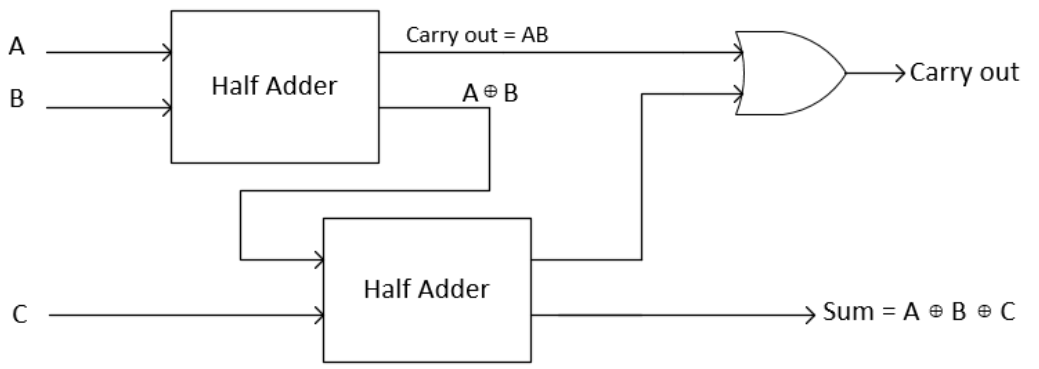
\includegraphics[width=1.1\linewidth]{Figuras/Ch9/somadorcompletomeio.PNG}}
}

\frame{
	\frametitle{Circuitos subtratores - Meio subtrator}

	\begin{block}{Meio Subtrator}
		\begin{itemize}
			\item Possibilita a subtração de 2 números binários de 1 bit.
			\item Entradas: 2 bits.
			\item Saídas: Diferença + \textit{Borrow}.
		\end{itemize}
	\end{block}

	\bigskip
	
%	\renewcommand{\arraystretch}{1}
	\centering
	\begin{adjustbox}{totalheight=0.6\textheight-2\baselineskip}
	\begin{tabular}{cc|cc}
		\toprule
		$ A $ & $ B $ & $ D $ & $ B_o $ \\ \midrule%\cmidrule(r{0.8em}){1-2}\cmidrule(l{-0.4em}){3-4}
		0 & 0 & 0 & 0   \\
		0 & 1 & 1 & 1   \\
		1 & 0 & 1 & 0   \\
		1 & 1 & 0 & 0   \\ \bottomrule
	\end{tabular}
	\end{adjustbox}
}

\frame{
	\frametitle{Circuitos subtratores - Meio subtrator}
	\setmyunit{2cm}
	
	\centering
	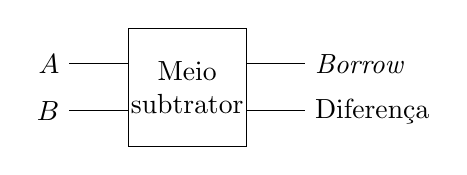
\begin{tikzpicture}[scale=1.5]
	\draw (0,0) rectangle node[text width=1.5cm, align=center] {Meio subtrator} ++(1,1);
	\draw (-0.5,0.3) node[left] {$ B $} -- ++(0.5,0) (-0.5,0.7) node[left] {$ A $} -- ++(0.5,0) (1,0.3) -- ++(0.5,0) node[right] {Diferença} (1,0.7) -- ++(0.5,0) node[right] {\textit{Borrow}};
	\end{tikzpicture}
}

\frame{
\frametitle{Circuitos subtratores - Meio subtrator}

\begin{center}

\begin{karnaugh-map}[2][2][1][$A$][$B$]
\manualterms{0,1,1,0}
\implicant{1}{1}
\implicant{2}{2}
\end{karnaugh-map}
\end{center}

\vspace{-0.5cm}

\begin{block}{Expressão simplificada}
	\[ D = {\color{orange} A \oplus B } \]
\end{block}
}

\frame{
\frametitle{Circuitos subtratores - Meio subtrator}

\begin{center}

\begin{karnaugh-map}[2][2][1][$A$][$B$]
\manualterms{0,0,1,0}
\implicant{2}{2}
\end{karnaugh-map}
\end{center}

\vspace{-0.5cm}

\begin{block}{Expressão simplificada}
	\[ B_o = {\color{red} \notted{A}\cdot B} \]
\end{block}
}

\frame{
	\frametitle{Circuitos subtratores - Meio subtrator}
	\setmyunit{2cm}
	
	\centering
	\begin{circuitikz}
		\node[xor port] (xor1) at (0,0) {};
		\node[and port] (and1) at (0,-1) {};
		\node[not port,scale=0.5] (not1) at ($ (and1.in 2)+(-0.5,0) $) {};
		
		\draw (xor1.in 1) to[short,-*] ++(-0.8,0) -- ++(-0.2,0) node[left] {$ A $} (xor1.in 2) to[short, -*] ++(-0.5,0) -- ++(-0.5,0) node[left] {$ B $} (xor1.in 1) ++(-0.8,0) |- (not1.in) (not1.out) -- (and1.in 2) (xor1.in 2) ++(-0.5,0) |- (and1.in 1) (xor1.out) -- ++(0.5,0) node[right] {$ D $} (and1.out) -- ++(0.5,0) node[right] {$ B $};
	\end{circuitikz}
%	\centerline{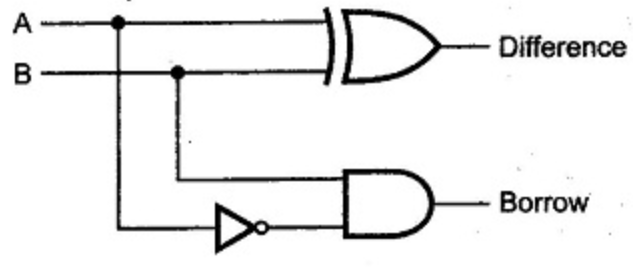
\includegraphics[width=0.9\linewidth]{Figuras/Ch9/meiosubtrator.PNG}}
}

\frame{
	\frametitle{Circuitos subtratores - Subtrator completo}
	\begin{block}{Subtrator Completo}
		\begin{itemize}
			\item Possibilita a soma de 2 números binários de 1 bit + o borrow anterior.
			\item Entradas: 2 bits + \textit{Borrow} anterior.
			\item Saídas: Diferença + \textit{Borrow}.
		\end{itemize}
	\end{block}

	\bigskip

	\centering
	\begin{tabular}{ccc|cc}
		\toprule
		$ A $ & $ B $ & $ B_{in} $ & $ D $ & $ B_{out} $ \\ \midrule%\cmidrule(r{1.4em}){1-3}\cmidrule(l{-0.2em}){4-5}
		0 & 0 & 0 & 0 & 0 \\
		0 & 0 & 1 & 1 & 1 \\
		0 & 1 & 0 & 1 & 1 \\
		0 & 1 & 1 & 0 & 1 \\
		1 & 0 & 0 & 1 & 0 \\
		1 & 0 & 1 & 0 & 0 \\
		1 & 1 & 0 & 0 & 0 \\
		1 & 1 & 1 & 1 & 1 \\ \bottomrule
	\end{tabular}

}

\frame{
	\frametitle{Circuitos subtratores - Subtrator completo}
	\setmyunit{2cm}
	
	\centering
	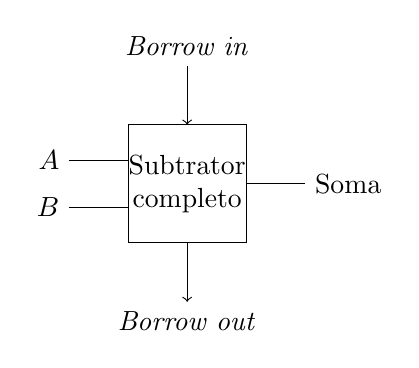
\begin{tikzpicture}[scale=1.5]
	\draw (0,0) rectangle node[text width=1.5cm, align=center] {Subtrator completo} ++(1,1);
	\draw (-0.5,0.3) node[left] {$ B $} -- ++(0.5,0) (-0.5,0.7) node[left] {$ A $} -- ++(0.5,0) (1,0.5) -- ++(0.5,0) node[right] {Soma};
	\draw[->] (0.5,1.5) node[above] {\textit{Borrow in}} -- ++(0,-0.5);
	\draw[->] (0.5,0) -- ++(0,-0.5) node[below] {\textit{Borrow out}};
	\end{tikzpicture}
}

\frame{
\frametitle{Circuitos subtratores - Subtrator completo}

\begin{center}

\begin{karnaugh-map}[4][2][1][$AB$][$B_{in}$]
\manualterms{0,1,1,0,1,0,0,1}
\implicant{1}{1}
\implicant{2}{2}
\implicant{4}{4}
\implicant{7}{7}
\end{karnaugh-map}
\end{center}

\vspace{-0.5cm}

\begin{block}{Expressão simplificada}
	\[ D = {\color{orange} A \oplus B \oplus B_{in}} \]
\end{block}
}

\frame{
\frametitle{Circuitos subtratores - Subtrator completo}

\begin{center}

\begin{karnaugh-map}[4][2][1][$AB$][$B_{in}$]
\manualterms{0,1,0,0,1,1,0,1}
\implicant{1}{5}
\implicant{4}{5}
\implicant{5}{7}
\end{karnaugh-map}
\end{center}

\vspace{-0.5cm}

\begin{block}{Expressão simplificada}
	\[ B_{out} = {\color{red} \notted{A}\cdot B} + {\color{green} \notted{A}\cdot B_{in}} + {\color{YellowOrange} B\cdot B_{in}} \]
\end{block}
}

\frame{
	\frametitle{Circuitos subtratores - Subtrator completo}
	\setmyunit{2cm}
	
	\centering
	\begin{circuitikz}
		\node[xor port] (xor1) at (0.5,0) {};
		\node[and port] (and1) at (0.5,-1) {};
		\node[and port] (and2) at (0.5,-1.75) {};
		\node[and port] (and3) at (0.5,-2.5) {};
		
		\node[xor port] (xor2) at (1.5,-0.25) {};
		\node[or port,number inputs=3] (or1) at (1.5,-1.75) {};
		
		\coordinate (a) at (-1.5,0.5);
		\coordinate (b) at (-1.1,0.5);
		\coordinate (c) at (-0.7,0.5);
		
		\node[not port,rotate=-90,scale=0.5] (not1) at ($ (a)+(0,-0.75) $) {};
		
		\draw (a) node[above] {$ A $} to[short,-*] (a|-xor1.in 1) -- (xor1.in 1) (a) -- (not1.in) (not1.out) |- (and2.in 1) (not1.out) to[short,-*] (not1.out|-and1.in 1) (xor1.in 1) -- (not1.out|-xor1.in 1) (and1.in 1) -- (a|-and1.in 1)
		(b) node[above] {$ B $} |- (and3.in 1) (b|-xor1.in 2) to[short, *-*] (b|-and1.in 2) (xor1.in 2) -- (b|-xor1.in 2) (and1.in 2) -- (b|-and1.in 2)
		(c) node[above] {$ B_{in} $} |- (and3.in 2) (c|-xor2.in 2) to[short,*-*] (c|-and2.in 2) (xor2.in 2) -- (c|-xor2.in 2) (and2.in 2) -- (c|-and2.in 2)
		(xor1.out) |- (xor2.in 1)
		(and1.out) -| (or1.in 1)
		(and2.out) -- (or1.in 2)
		(and3.out) -| (or1.in 3)
		(xor2.out) -- ++(0.5,0) node[right] {$ S $}
		(or1.out) -- ++(0.5,0) node[right] {$ B_{out} $};
	\end{circuitikz}
%	\centerline{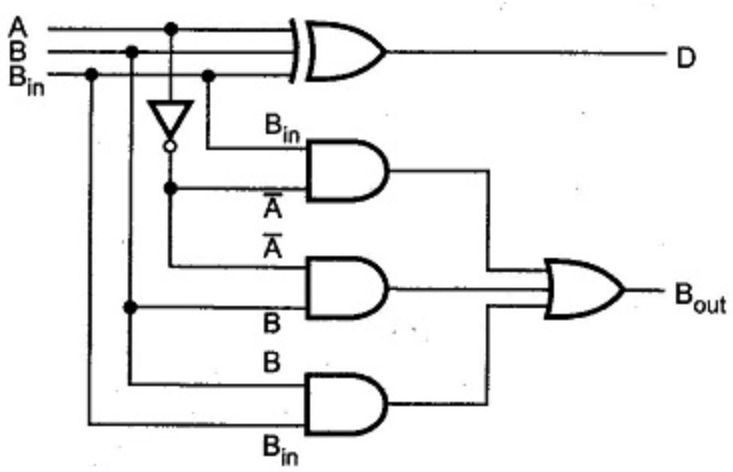
\includegraphics[width=0.75\linewidth]{Figuras/Ch9/subtratorcompleto.PNG}}
}

\frame{
	\frametitle{Circuitos subtratores - Subtrator de $ n $ bits}
	\begin{block}{\textbf{Ex.:} Subtrator de 4 bits}
		\begin{itemize}
			\item Utiliza-se 4 subtratores completos, um para cada bit.
			\item Conecta-se cada $B_{out}$ no $B_{in}$ do próximo bit.
		\end{itemize}
	\end{block}

	\centerline{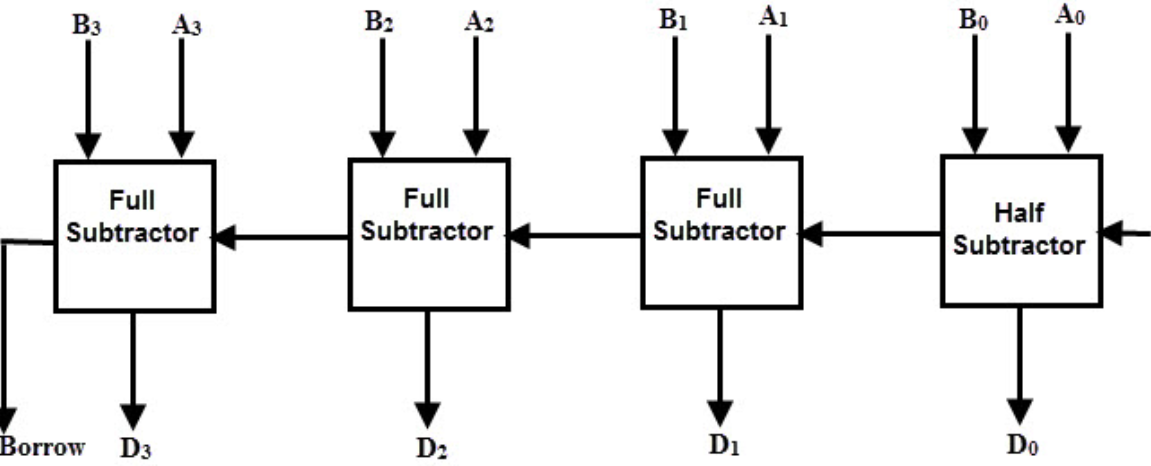
\includegraphics[width=0.9\linewidth]{Figuras/Ch9/subtratornbits.PNG}}
}

\frame{
	\frametitle{Circuitos subtratores - Subtrator completo a partir de meio subtratores}
	\begin{block}{}
		\begin{itemize}
			\item Meio subtrator:
			\begin{align*}
				D 		&= {\color{orange} A \oplus B_{in}}\\
				B_{out} &= {\color{red} \notted{A}\cdot B}
			\end{align*}
			\item Subtrator completo:
			\begin{align*}
				D 		&= {\color{orange} A \oplus B \oplus B_{in}}\\
				B_{out} &= \notted{A}\cdot B\cdot \notted{B_{in}} + \notted{A}\cdot \notted{B}\cdot B_{in} + \notted{A}\cdot B\cdot B_{in} + A\cdot B\cdot B_{in}\\
						&= {\color{red} B_{in}\notted{(A \oplus B)} + \notted{A}\cdot B}
			\end{align*}
		\end{itemize}
	\end{block}

}

\frame{
	\frametitle{Circuitos subtratores - Subtrator completo a partir de meio subtratores}
	\setmyunit{2cm}
	
	\centering
	\begin{circuitikz}
		\node[xor port] (xor1) at (1,0) {};
		\node[and port] (and1) at (1,-0.75) {};
		\node[not port,scale=0.5] (not1) at ($ (and1.in 2)+(-0.5,0) $) {};
		
		\node[xor port] (xor2) at (3,-0.14) {};
		\node[and port] (and2) at (3,-0.875) {};
		\node[not port,scale=0.5] (not2) at ($ (and2.in 2)+(-0.5,0) $) {};
		
		\node[or port] (or1) at (4,-1.015) {};
		
		\coordinate (a) at ($ (xor1.in 1)+(-1,0) $);
		\coordinate (b) at ($ (xor1.in 2)+(-1,0) $);
		\coordinate (c) at ($ (and1.in 2)+(-1,-0.5) $);
		
		\draw (a) node[left] {$ A $};
		\draw (b) node[left] {$ B $};
		\draw (c) node[left] {$ B_{in} $};
		
		\draw (a) to[short,-*] ++(0.2,0) |- (not1.in) (not1.out) -- (and1.in 2) (a) -- (xor1.in 1)
		(b) to[short,-*] ++(0.4,0) |- (and1.in 1) (b) -- (xor1.in 2)
		(xor1.out) -- (xor2.in 1) (xor1.out) to[short,-*] ++(0.5,0) |- (not2.in) (not2.out) -- (and2.in 2);
		
		\coordinate (p1) at ($ (xor1.out)+(0.3,0) $);
		
		\draw (c) -- (p1|-c) -- (xor2.in 2-|p1) -- (xor2.in 2) to[short,-*] ++(-0.3,0) |- (and2.in 1) 
		(and1.out) -- ++(0,-0.5) -| (or1.in 2)
		(and2.out) -- (or1.in 1)
		(xor2.out) -- ++(1.1,0) node[right] {$ D $}
		(or1.out) -- ++(0.1,0) node[right] {$ B_{out} $};
		
		\draw[dashed,gray] ($ (a)+(0.1,0.2) $) rectangle ($ (and1.out)+(0.1,-0.35) $) node[midway,below=0.75,black] {Meio subtrator};
		
		\draw[dashed,gray] ($ (p1)+(-0.1,0.2) $) rectangle ($ (and2.out)+(0.1,-0.35) $) node[midway,above=0.7,black] {Meio subtrator};
	\end{circuitikz}
%	\centerline{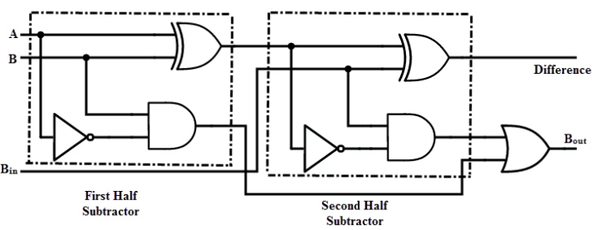
\includegraphics[width=1.1\linewidth]{Figuras/Ch9/subtratorcompletomeio.png}}
}


\section*{Exercícios}

\frame{
	\frametitle{Exercícios}
	\begin{block}{}
		01. Projete um circuito combinacional que realize as duas operações - somador e subtrator. Para tal, acrescente uma variável de entrada \textbf{M} que faça este controle. Assuma que para $M = 0$, o circuito realize uma soma completa.\newline \\

		02. Desenhe um sistema somador para dois números de dois bits apenas com blocos de somadores completos.
	\end{block}
}

\section*{Referências}


\frame{
	\frametitle{Referências e exercícios complementares}
	\begin{itemize}
		\item IDOETA, Ivan V. e CAPUANO, Francisco G. Elementos de Eletrônica Digital. São Paulo:
		      Editora Érica, ed. 40. 2008.
	\end{itemize}

	\centering{\alert{Página 229 - \textbf{5.6.10 até 5.6.17}}}

}